\section{Riemann and Darboux Integration} 

  We have done integration over closed intervals $[a, b]$. The natural extension is to define integration over \textit{boxes} $B = \prod_i [a_i, b_i]$. Essentially the construction is exactly the same. 

  \begin{definition}[Partition/Mesh]
    Let $B = \prod_i [a_i, b_i] \subset \mathbb{R}^n$ be a box. Then, a \textbf{partition}---or \textbf{mesh}---of $B$ is a finite set of points $P = \{x_{ij}\}_{1 \leq i \leq n, 0 \leq j \leq m_i}$\footnote{Therefore, for each dimension $i$, we want to take the interval $[a_i, b_i]$ and subdivide it into $m_i+1$ subintervals.} s.t. 
    \begin{equation}
      a_i = x_{i, 0} \leq x_{i, 1} \leq x_{i, 2} \leq \ldots \leq x_{i, m_i-1} \leq x_{i, m_i} = b \quad \forall i = 1, \ldots, n
    \end{equation}
    We denote each \textbf{box} within the partition as 
    \begin{equation}
      \Delta_J = \Delta_{j_1, j_2, \ldots, j_n} = \prod_{i} [x_{i, j_k-1}, x_{i, j_k}] \quad \forall j_i = 1, \ldots, m_i
    \end{equation}
    of volume $|\Delta_J| \coloneqq \prod_{i} (x_{i, j_k} - x_{i, j_{k-1}})$. 
  \end{definition}

  This nearly\footnote{since boundaries overlap} partitions $B$ into a grid of $\prod_i m_i$ smaller boxes, and can be seen as a discretization of the integral which we will construcct. 

  \begin{definition}[Riemann Sums with Respect to Partition]
    Let $P$ be a partition of $B \in \mathbb{R}^n$ and let $f: B \subset \mathbb{R}^n \to \mathbb{R}$ be bounded. Then, the \textbf{upper and lower Riemann sums} of $f$ with respect to $P$ are defined 
    \begin{equation}
      U(P, f) \coloneqq \sum_{J} \sup_{x \in \Delta_J} f(x) |\Delta_J|, \qquad L(P, f) \coloneqq \sum_{J} \inf_{x \in \Delta_J} f(x) |\Delta_J|
    \end{equation}

    \begin{figure}[H]
      \centering
      \begin{subfigure}[b]{0.48\textwidth}
        \centering
        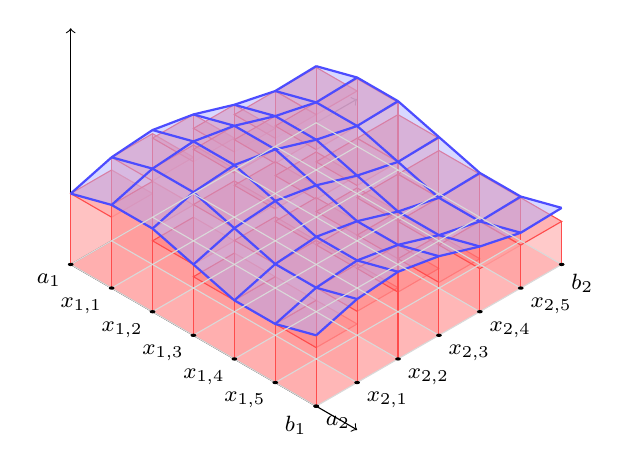
\begin{tikzpicture}[scale=0.6,
          x={(0.866cm,-0.5cm)}, y={(0.866cm,0.5cm)}, z={(0cm,1cm)}]
          
          % Draw axes (without labels)
          \draw[->] (0,0,0) -- (7,0,0);
          \draw[->] (0,0,0) -- (0,7,0);
          \draw[->] (0,0,0) -- (0,0,5);
          
          % Draw rectangular prisms (lower Riemann sum)
          % Using minimum z-value in each cell for lower sum
          \foreach \x in {0,1,2,3,4,5} {
            \foreach \y in {0,1,2,3,4,5} {
              % Calculate heights at four corners of the cell
              \pgfmathsetmacro{\zaa}{1.5 + 0.3*sin(\x*60) + 0.35*sin(\y*50)}
              \pgfmathsetmacro{\zba}{1.5 + 0.3*sin((\x+1)*60) + 0.35*sin(\y*50)}
              \pgfmathsetmacro{\zbb}{1.5 + 0.3*sin((\x+1)*60) + 0.35*sin((\y+1)*50)}
              \pgfmathsetmacro{\zab}{1.5 + 0.3*sin(\x*60) + 0.35*sin((\y+1)*50)}
              
              % Find minimum height (lower Riemann sum)
              \pgfmathsetmacro{\zmin}{min(\zaa,min(\zba,min(\zbb,\zab)))}
              
              % Bottom face (on xy-plane)
              \fill[red!30, opacity=0.6] (\x,\y,0) -- (\x+1,\y,0) -- (\x+1,\y+1,0) -- (\x,\y+1,0) -- cycle;
              
              % Front face
              \fill[red!40, opacity=0.6] (\x,\y,0) -- (\x+1,\y,0) -- (\x+1,\y,\zmin) -- (\x,\y,\zmin) -- cycle;
              
              % Right face
              \fill[red!35, opacity=0.6] (\x+1,\y,0) -- (\x+1,\y+1,0) -- (\x+1,\y+1,\zmin) -- (\x+1,\y,\zmin) -- cycle;
              
              % Top face
              \fill[red!50, opacity=0.6] (\x,\y,\zmin) -- (\x+1,\y,\zmin) -- (\x+1,\y+1,\zmin) -- (\x,\y+1,\zmin) -- cycle;
              
              % Draw edges
              \draw[red!70] (\x,\y,0) -- (\x,\y,\zmin);
              \draw[red!70] (\x+1,\y,0) -- (\x+1,\y,\zmin);
              \draw[red!70] (\x+1,\y+1,0) -- (\x+1,\y+1,\zmin);
              \draw[red!70] (\x,\y+1,0) -- (\x,\y+1,\zmin);
              \draw[red!70] (\x,\y,\zmin) -- (\x+1,\y,\zmin) -- (\x+1,\y+1,\zmin) -- (\x,\y+1,\zmin) -- cycle;
            }
          }
          
          % Draw surface patches first (back to front for proper layering)
          \foreach \ystart/\yend in {0/1, 1/2, 2/3, 3/4, 4/5, 5/6} {
            \foreach \xstart/\xend in {0/1, 1/2, 2/3, 3/4, 4/5, 5/6} {
              \pgfmathsetmacro{\zaa}{1.5 + 0.3*sin(\xstart*60) + 0.35*sin(\ystart*50)}
              \pgfmathsetmacro{\zba}{1.5 + 0.3*sin(\xend*60) + 0.35*sin(\ystart*50)}
              \pgfmathsetmacro{\zbb}{1.5 + 0.3*sin(\xend*60) + 0.35*sin(\yend*50)}
              \pgfmathsetmacro{\zab}{1.5 + 0.3*sin(\xstart*60) + 0.35*sin(\yend*50)}
              
              \fill[blue!30, opacity=0.5] 
                (\xstart,\ystart,\zaa) --
                (\xend,\ystart,\zba) --
                (\xend,\yend,\zbb) --
                (\xstart,\yend,\zab) -- cycle;
            }
          }
          
          % Draw grid lines on surface
          % Lines parallel to x-axis
          \foreach \y in {0,1,2,3,4,5,6} {
            \draw[blue!70, thick] 
              (0,\y,{1.5 + 0.35*sin(\y*50)}) 
              \foreach \x in {1,2,3,4,5,6} {
                -- (\x,\y,{1.5 + 0.3*sin(\x*60) + 0.35*sin(\y*50)})
              };
          }
          
          % Lines parallel to y-axis
          \foreach \x in {0,1,2,3,4,5,6} {
            \draw[blue!70, thick] 
              (\x,0,{1.5 + 0.3*sin(\x*60)}) 
              \foreach \y in {1,2,3,4,5,6} {
                -- (\x,\y,{1.5 + 0.3*sin(\x*60) + 0.35*sin(\y*50)})
              };
          }
          
          % Base grid
          \foreach \x in {0,1,2,3,4,5,6} {
            \draw[gray!30, thin] (\x,0,0) -- (\x,6,0);
            \draw[gray!30, thin] (0,\x,0) -- (6,\x,0);
          }
          
          % X-axis tick labels (back axis)
          \foreach \x/\label in {0/a_1, 1/x_{1,1}, 2/x_{1,2}, 3/x_{1,3}, 4/x_{1,4}, 5/x_{1,5}, 6/b_1} {
            \fill (\x,0,0) circle (0.05);
            \node[below left, font=\footnotesize] at (\x,0,0) {$\label$};
          }
          
          % Y-axis tick labels (front axis at x=6)
          \foreach \y/\label in {0/a_2, 1/x_{2,1}, 2/x_{2,2}, 3/x_{2,3}, 4/x_{2,4}, 5/x_{2,5}, 6/b_2} {
            \fill (6,\y,0) circle (0.05);
            \node[below right, font=\footnotesize] at (6,\y,0) {$\label$};
          }
        \end{tikzpicture}
        \caption{Lower Riemann sum.}
        \label{fig:lower_riemann_sum}
      \end{subfigure}
      \hfill 
      \begin{subfigure}[b]{0.48\textwidth}
        \centering
        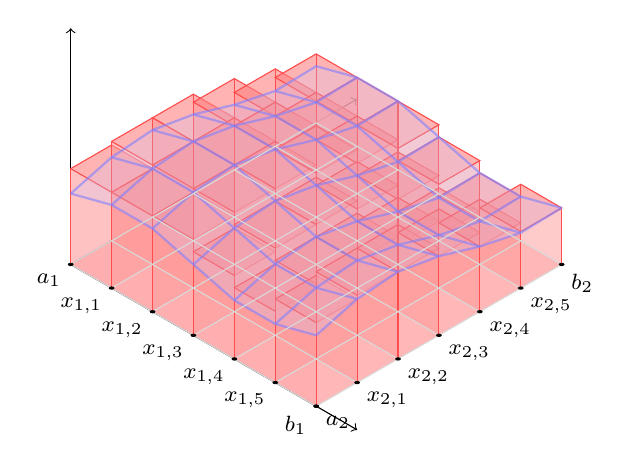
\begin{tikzpicture}[scale=0.6,
          x={(0.866cm,-0.5cm)}, y={(0.866cm,0.5cm)}, z={(0cm,1cm)}]
          
          % Draw axes (without labels)
          \draw[->] (0,0,0) -- (7,0,0);
          \draw[->] (0,0,0) -- (0,7,0);
          \draw[->] (0,0,0) -- (0,0,5);
          
          % Draw rectangular prisms (upper Riemann sum)
          % Using maximum z-value in each cell for upper sum
          \foreach \x in {0,1,2,3,4,5} {
            \foreach \y in {0,1,2,3,4,5} {
              % Calculate heights at four corners of the cell
              \pgfmathsetmacro{\zaa}{1.5 + 0.3*sin(\x*60) + 0.35*sin(\y*50)}
              \pgfmathsetmacro{\zba}{1.5 + 0.3*sin((\x+1)*60) + 0.35*sin(\y*50)}
              \pgfmathsetmacro{\zbb}{1.5 + 0.3*sin((\x+1)*60) + 0.35*sin((\y+1)*50)}
              \pgfmathsetmacro{\zab}{1.5 + 0.3*sin(\x*60) + 0.35*sin((\y+1)*50)}
              
              % Find maximum height (upper Riemann sum)
              \pgfmathsetmacro{\zmax}{max(\zaa,max(\zba,max(\zbb,\zab)))}
              
              % Bottom face (on xy-plane)
              \fill[red!30, opacity=0.6] (\x,\y,0) -- (\x+1,\y,0) -- (\x+1,\y+1,0) -- (\x,\y+1,0) -- cycle;
              
              % Front face
              \fill[red!40, opacity=0.6] (\x,\y,0) -- (\x+1,\y,0) -- (\x+1,\y,\zmax) -- (\x,\y,\zmax) -- cycle;
              
              % Right face
              \fill[red!35, opacity=0.6] (\x+1,\y,0) -- (\x+1,\y+1,0) -- (\x+1,\y+1,\zmax) -- (\x+1,\y,\zmax) -- cycle;
              
              % Top face
              \fill[red!50, opacity=0.6] (\x,\y,\zmax) -- (\x+1,\y,\zmax) -- (\x+1,\y+1,\zmax) -- (\x,\y+1,\zmax) -- cycle;
              
              % Draw edges
              \draw[red!70] (\x,\y,0) -- (\x,\y,\zmax);
              \draw[red!70] (\x+1,\y,0) -- (\x+1,\y,\zmax);
              \draw[red!70] (\x+1,\y+1,0) -- (\x+1,\y+1,\zmax);
              \draw[red!70] (\x,\y+1,0) -- (\x,\y+1,\zmax);
              \draw[red!70] (\x,\y,\zmax) -- (\x+1,\y,\zmax) -- (\x+1,\y+1,\zmax) -- (\x,\y+1,\zmax) -- cycle;
            }
          }
          
          % Draw surface patches with lighter opacity
          \foreach \ystart/\yend in {0/1, 1/2, 2/3, 3/4, 4/5, 5/6} {
            \foreach \xstart/\xend in {0/1, 1/2, 2/3, 3/4, 4/5, 5/6} {
              \pgfmathsetmacro{\zaa}{1.5 + 0.3*sin(\xstart*60) + 0.35*sin(\ystart*50)}
              \pgfmathsetmacro{\zba}{1.5 + 0.3*sin(\xend*60) + 0.35*sin(\ystart*50)}
              \pgfmathsetmacro{\zbb}{1.5 + 0.3*sin(\xend*60) + 0.35*sin(\yend*50)}
              \pgfmathsetmacro{\zab}{1.5 + 0.3*sin(\xstart*60) + 0.35*sin(\yend*50)}
              
              \fill[blue!20, opacity=0.25] 
                (\xstart,\ystart,\zaa) --
                (\xend,\ystart,\zba) --
                (\xend,\yend,\zbb) --
                (\xstart,\yend,\zab) -- cycle;
            }
          }
          
          % Draw grid lines on surface (lighter)
          % Lines parallel to x-axis
          \foreach \y in {0,1,2,3,4,5,6} {
            \draw[blue!50, thick, opacity=0.6] 
              (0,\y,{1.5 + 0.35*sin(\y*50)}) 
              \foreach \x in {1,2,3,4,5,6} {
                -- (\x,\y,{1.5 + 0.3*sin(\x*60) + 0.35*sin(\y*50)})
              };
          }
          
          % Lines parallel to y-axis
          \foreach \x in {0,1,2,3,4,5,6} {
            \draw[blue!50, thick, opacity=0.6] 
              (\x,0,{1.5 + 0.3*sin(\x*60)}) 
              \foreach \y in {1,2,3,4,5,6} {
                -- (\x,\y,{1.5 + 0.3*sin(\x*60) + 0.35*sin(\y*50)})
              };
          }
          
          % Base grid
          \foreach \x in {0,1,2,3,4,5,6} {
            \draw[gray!30, thin] (\x,0,0) -- (\x,6,0);
            \draw[gray!30, thin] (0,\x,0) -- (6,\x,0);
          }
          
          % X-axis tick labels (back axis)
          \foreach \x/\label in {0/a_1, 1/x_{1,1}, 2/x_{1,2}, 3/x_{1,3}, 4/x_{1,4}, 5/x_{1,5}, 6/b_1} {
            \fill (\x,0,0) circle (0.05);
            \node[below left, font=\footnotesize] at (\x,0,0) {$\label$};
          }
          
          % Y-axis tick labels (front axis at x=6)
          \foreach \y/\label in {0/a_2, 1/x_{2,1}, 2/x_{2,2}, 3/x_{2,3}, 4/x_{2,4}, 5/x_{2,5}, 6/b_2} {
            \fill (6,\y,0) circle (0.05);
            \node[below right, font=\footnotesize] at (6,\y,0) {$\label$};
          }
        \end{tikzpicture}
        \caption{Upper Riemann sum.}
        \label{fig:upper_riemann_rum}
      \end{subfigure}
      \caption{}
    \end{figure}
  \end{definition}

  \begin{definition}[Riemann Integral]
    Given that $f: B \subset \mathbb{R}^n \to \mathbb{R}$ is bounded, the \textbf{upper and lower Riemann integrals} of $f$ are defined 
    \begin{equation}
      \overline{\int_B} f(x) \,dx \coloneqq \inf_P U(P, f), \qquad \underline{\int_B} f(x) \,dx \coloneqq \sup_P L(P, f) 
    \end{equation}
    If the upper and lower Riemann integrals are equal, then the \textbf{Riemann integral} of $f$ 
    \begin{equation}
      \int_B f(x) \,dx 
    \end{equation}
    is defined as such. Furthermore, $f$ is said to be \textbf{Riemann integrable} over $B$. 
  \end{definition} 

\subsection{Conditions for Integrability} 

  \begin{theorem}[]
    $f: B \subset \mathbb{R}^n \to \mathbb{R}$ continuous means $f$ is integrable over $B$. 
  \end{theorem}

  However, there are some functions with discontinuities that are in fact integrable. 
  \begin{enumerate}
    \item Given that there is a subset $N$ in $B$ with volume $0$ over which $f$ is not defined, we can integrate over $B \setminus N$. In the one and two dimensional cases, 
    \[\int_{B \setminus N} f(x) dx \text{ and } \iint_{B\setminus N} f(x) dA\]
    are well-defined. Visually, 
    \begin{center}
      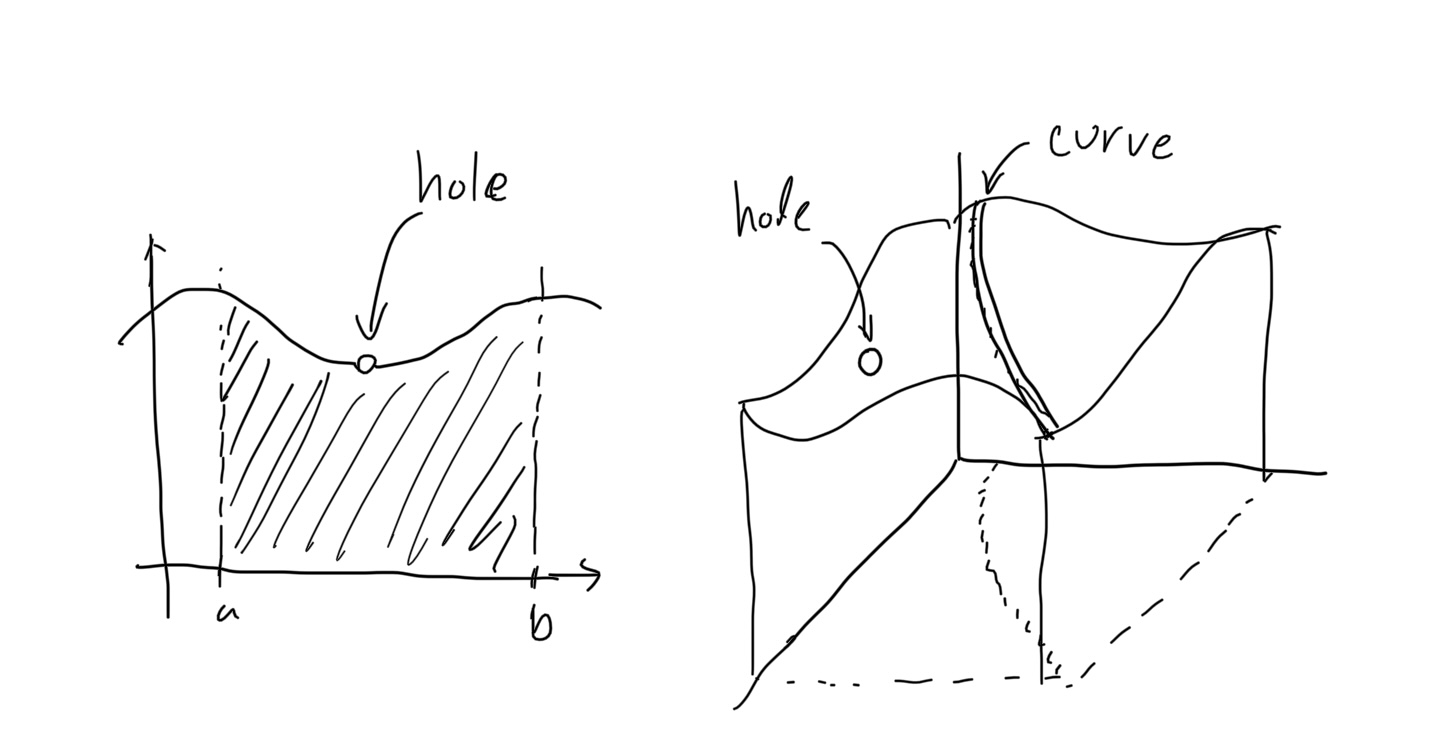
\includegraphics[scale=0.2]{img/Integrable_Hole_Function.jpg}
    \end{center}
    \item The function is defined for all values in the region, but there is a jump in the value of the function. 
    \begin{center}
      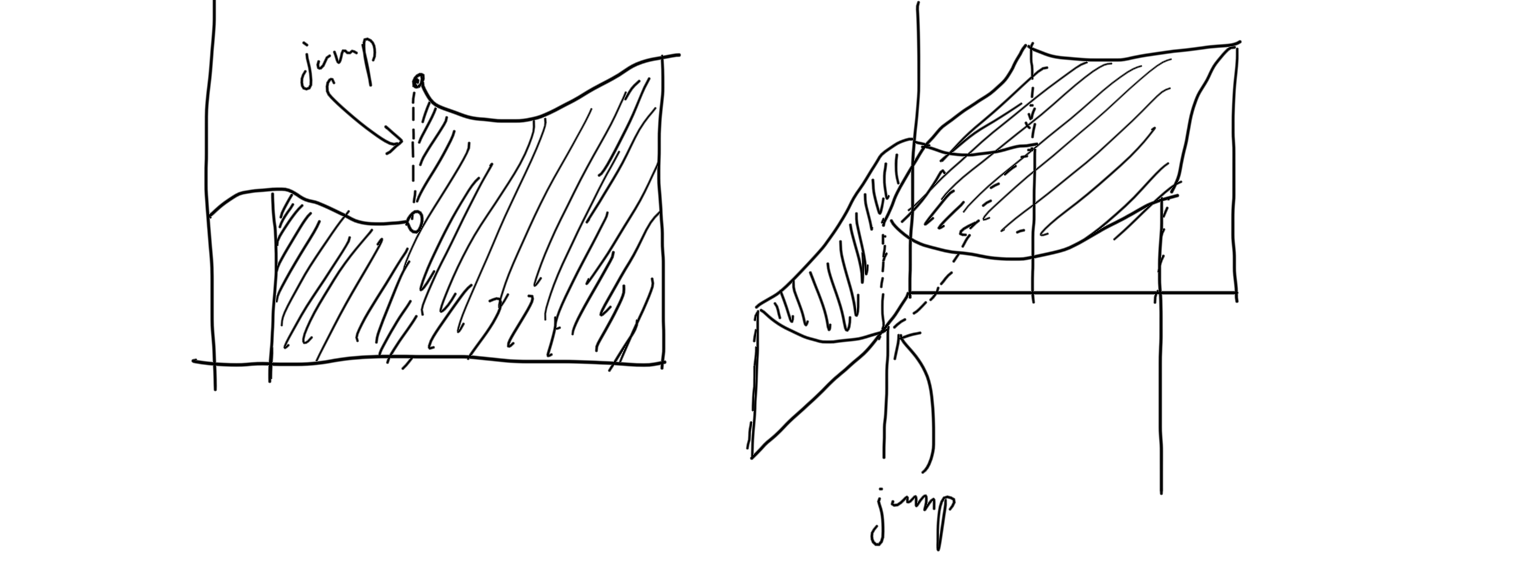
\includegraphics[scale=0.23]{img/Integrable_Jump_Function.PNG}
    \end{center}
  \end{enumerate}
  Informally, if we can visualize the Riemann sum converging to a well-defined area as the rectangles get thinner and thinner, then a discontinuous function is integrable. Indeed, all continuous functions (over a bounded set) are integrable since their Riemann sums are well defined. 


\subsection{Iterated Integrals and Fubini's Theorem} 

  The construction of the integral is one step, but we should know how to practically compute such an integral. We can do this by recursively ``reducing'' the dimension of the region of the integral until we can work with one dimension. This is known as \textit{Cavalieri's principle}: Let $S$ be a bounded $n$-dimensional solid in $\mathbb{R}^n$. Define an $n-1$ subspace $P$ in $\mathbb{R}^n$ and given the quotient space $\mathbb{R}^n / P$ with elements $P_x$, let 
  \begin{equation}
    S \subset \bigcup_{a \leq x \leq b} P_x
  \end{equation}
  That is, $S$ is "in between" affine subspaces $P_a$ and $P_b$. Given the cross section of $S$ with $P_x$, defined $P_x \cap S$, denote the integral of this cross section as $A(x)$. Then, colloquially, the volume of $S$ can be represented as the integral $\int_a^b A(x)\,dx$. This idea basically says that the volume of $S$ is the sum of the areas of its infinitesimal cross sections. 

  \begin{figure}[H]
    \centering 
    
\includegraphics[scale=0.27]{img/Cavalieri_Principle.PNG}
    \caption{Visual of Cavalieri's principle.} 
    \label{fig:cavalieri}
  \end{figure}

  Given a solid $S \subset \mathbb{R}^n$, it is easy to see that no matter what subspace $P$ we choose–that is, no matter what orientation we choose to "cut" the solid– the sum of all of its cross sections should be equal to the true volume of $S$. In the case when $S$ is a box in $\mathbb{R}^n$, Fubini's theorem states that whether we cut $S$ up along the $x_1$-axis, $x_2$-axis, ..., or the $x_n$-axis, the symmetry in volume is always preserved. This theorem is really just a specific case of this general symmetry in volume. 

  \begin{theorem}[Fubini's Theorem]
    Given a function $f: \mathbb{R}^n \longrightarrow \mathbb{R}$, let 
    \[B \equiv \prod_{i=1}^n [\alpha_i, \beta_i]\]
    and let 
    $p$ be any permutation of the elements $\{x_1, x_2, ..., x_n\}$. Then 
    \begin{align*}
        \int_B f \; d V & = \int_{\alpha_n}^{\beta_n} ... \int_{\alpha_1}^{\beta_1} f(x_1,x_2,...,x_n) \; d x_1 ... d x_n \\
        & = \int_{p(\alpha_n)}^{p(\beta_n)} ... \int_{p(\alpha_1)}^{p(\beta_1)} f(x_1,x_2, ..., x_n) \; d p(x_1) ... d p(x_n) 
    \end{align*}
    In the two dimensional case, we have
    \begin{align*}
        \iint_B f \; d A & = \int_c^d \int_a^b f(x, y) \; d x \, d y = \int_a^b \int_c^d f(x, y) \; d y \, d x 
    \end{align*}
    \begin{center}
        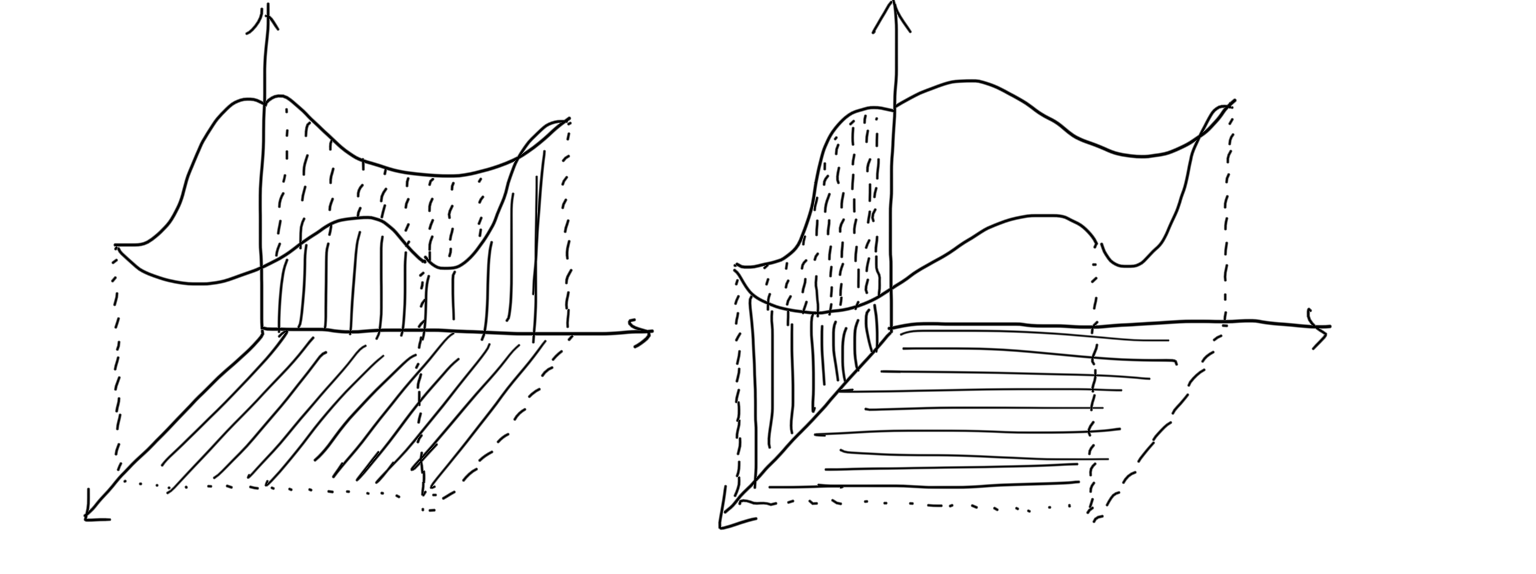
\includegraphics[scale=0.27]{img/Fubini_Theorem.PNG}
    \end{center}
    In the three dimensional case, we have
    \begin{align*}
        \iiint_B f \; d V & 
        = \int_e^f \int_c^d \int_a^b f(x, y, z) \; d x \, d y \, d z = \int_e^f \int_a^b \int_c^d f(x, y, z) \; d y \, d x \, d z \\
        & = \int_c^d \int_a^b \int_e^f f(x, y, z) \; d z \, d x \, d y = \int_c^d \int_e^f \int_a^b f(x, y, z) \; d x \, d z \, d y \\
        & = \int_a^b \int_e^f \int_c^d f(x, y, z) \; d y \, d z \, d x = \int_a^b \int_c^d \int_e^f f(x, y, z) \; d z \, d y \, d x 
    \end{align*}
  \end{theorem}

  Computation of these integrals is simple. You do the innermost integral first with respect to the corresponding variable, while treating the rest of the variables constant. Evaluating each integral outputs a formula for a higher dimensional cross section of the solid $S$. It is clear that computing iterated integrals is really just doing Cavalieri's principle repeatedly. 

\subsection{Integration over Regions between Curves} 

  \begin{definition}[Simple Regions w.r.t. a Variable]
    A bounded region $D$ in $\mathbb{R}^n$ is said to be $x_i$-simple if it is bounded by the graphs of two continuous functions $u_1, u_2: \mathbb{R}^{n-1} \longrightarrow \mathbb{R}$ of the variables 
    \[x_1, x_2, ..., x_{i-1}, x_{i+1}, ..., x_n\]
    That is, $D$ can be expressed in the form 
    \[\{ x \in \mathbb{R}^n \; | \; u_1 (x_1,..., x_{i-1}, x_{i+1}, ... , x_n) \leq x_i \leq u_2 (x_1, ..., x_{i-1}, x_{i+1}, ..., x_n)\}\]
    If a region is simple in all of its variables, it is simply called \textit{simple}. Note that $n$-dimensional boxes are simple regions. 
  \end{definition}

  \begin{example}
    In $\mathbb{R}^2$, the region on the left graph is an $y$-simple region and the region on the right is a $x$-simple region. 
    \begin{center}
    \begin{tikzpicture}[scale=0.8]
      \draw[<->] (-1,0)--(5,0);
      \draw[<->] (0,-1)--(0,5);
      \draw[<->] (6,0)--(12,0);
      \draw[<->] (7,-1)--(7,5);
      \draw plot [smooth] coordinates {(0.6, 1.2) (1,1) (2,1.4) (3,1.3) (4,1.5) (4.3,1.7)};
      \draw plot [smooth] coordinates {(0.6, 3.9) (1,4.1) (2,4) (3,4.3) (4,4.2) (4.3,4.1)};
      \draw[dashed] (0.6,1.2)--(0.6,3.9);
      \draw[dashed] (4.3,1.7)--(4.3,4.1);
      \draw plot [smooth] coordinates {(8.2,0.6) (8,1) (8.4,2) (8.3,3) (8.5,4) (8.7,4.3)};
      \draw plot [smooth] coordinates {(10.9,0.6) (11.1,1) (11,2) (11.3,3) (11.2,4) (11.1,4.3)};
      \draw[dashed] (8.2,0.6)--(10.9,0.6);
      \draw[dashed] (8.7,4.3)--(11.1,4.3);
      \node[below] at (4.8,0) {$x$};
      \node[below] at (11.8,0) {$x$};
      \node[left] at (0,4.8) {$y$};
      \node[left] at (7,4.8) {$y$};
      \node[above] at (3,4.2) {$u_1$};
      \node[above] at (3,1.3) {$u_2$};
      \node[left] at (8.3, 3) {$v_1$};
      \node[right] at (11.3, 3) {$v_2$};
      \draw[fill] (0.6,0) circle (0.05);
      \node[below] at (0.6,0) {$a$};
      \draw[fill] (4.3,0) circle (0.05);
      \node[below left] at (4.3,0) {$b$};
      \draw[fill] (7,0.6) circle (0.05);
      \draw[fill] (7,4.3) circle (0.05);
      \node[left] at (7,0.6) {$c$};
      \node[left] at (7,4.3) {$d$};
    \end{tikzpicture}
    \end{center}
  \end{example}

  We now describe the method of calculating double integrals over elementary regions. 
  \begin{theorem}
  The double integral over a $y$-simple region $D$ bounded by functions $u_1$ and $u_2$ in $\mathbb{R}^2$ and the $x$-values $a$ and $b$ (as shown in the left graph of example 2.1) is
  \[\iint_D f(x, y) = \int_a^b \int_{u_2 (x)}^{u_1 (x)} f(x, y) \, dy \, dx\]
  The double integral over an $x$-simple region $D$ bounded by functions $v_1$ and $v_2$ in $\mathbb{R}^2$ and the $y$-values $c$ and $d$ (shown in the right of graph of example 2.1) is 
  \[\iint_D f(x, y) = \int_c^d \int_{v_2 (y)}^{v_1 (y)} f(x, y) \, dx \, dy\]
  \end{theorem}

  \begin{example}
  Integrating $f(x, y)$ over the unit disk would have the form
  \[\int_{-1}^1 \int_{-\sqrt{1-x^2}}^{\sqrt{1-x^2}} f(x,y) \, dy\, dx \text{ or } \int_{-1}^1 \int_{-\sqrt{1-y^2}}^{\sqrt{1-y^2}} f(x,y) \, dx\, dy \]
  Note that the unit disk is both $x$ and $y$ simple. 
  \end{example}

\subsection{Change of Basis}

  Sometimes, integrating a region over a different basis would make the integral computation much more simpler. In this case, we may be able to transform more complicated regions into elementary regions. We first introduce a change of basis in 2 dimensions and then generalize it into higher dimensions. 
  
  Let $\mathbb{R}^2$ have the standard orthonomal basis $e_1, e_2$, commonly known as the $x, y$ basis. Now, let us construct new basis vectors of $\mathbb{R}^2$, denoted $f_1, f_2$ such that $f_1, f_2$ are functions of $e_1, e_2$. Since they are both bases that span $\mathbb{R}^2$, we can equally represent $e_1, e_2$ as functions of $f_1, f_2$. 
  \begin{align*}
      &e_1 = g(f_1, f_2)\\
      &e_2 = h(f_1, f_2) 
  \end{align*}
  Note that this change of basis does not necessarily have to be linear, as in the context of passive transformation in linear algebra. Then, every point $(x,y)$ in the $(e_1, e_2)$-basis can be rewritten as
  \begin{align*}
      (x, y) & = x e_1 + y e_2 \\
      & = x \, g(f_1, f_2) + y \, h(f_1, f_2) \\
      & = u f_1 + v f_2
  \end{align*}
  Note that it is customary to denote $x, y$ as the coefficients in the $e_1, e_2$ basis and $u, v$ as the coefficients in the new $f_1, f_2$ basis. This way, we can not only write $e_1$ and $e_2$ as functions of $f_1$ and $f_2$, but we can also write the coefficents $x, y$ as functions of the coeffiecents $u, v$! That is, 
  \begin{align*}
      & x = x(u, v) \\
      & y = y(u, v)
  \end{align*}
  which is really just a function 
  \[B: \mathbb{R}^2 \longrightarrow \mathbb{R}^2, \;\; B(u, v) = \begin{pmatrix} x(u, v) \\ y(u, v) \end{pmatrix}\]
  Notice that $B$ changes the $u, v$ coordinates to the $x, y$ coordinates, and $B^{-1}$ changes the $x, y$ coordinates to the $u, v$ coordinates. 
  \[B^{-1}: \mathbb{R}^2 \longrightarrow \mathbb{R}^2, \;\; B^{-1} (x, y) = \begin{pmatrix} u (x, y) \\ v (x, y) \end{pmatrix}\]
  Note that these coefficients actually change \textit{contravariantly}, that is, they change inversely with respect to how the basis vectors are changed. In vector calculus, it is conventional to represent a change of basis with functions that relate the coefficients $x, y$ with $u, v$, rather than the bases $f_1, f_2$ with $e_1, e_2$. 

  \begin{theorem}[Integration over Change of Bases in $\mathbb{R}^2$]
  Let $\mathbb{R}^2$ have the standard orthonomal basis $e_1, e_2$. Now, let us construct new basis vectors of $\mathbb{R}^2$, denoted $f_1, f_2$ such that the coefficients of the vectors in $\mathbb{R}^2$ are related by the change of basis function 
  \[B = \begin{pmatrix} x \\ y \end{pmatrix} \implies B(u, v) = \begin{pmatrix} x(u, v) \\ y(u, v) \end{pmatrix}\]
  Given region $D \subset \mathbb{R}^2$ and $S = B(D)$ is the region transformed by $B$, the integral of function $f(x, y)$ over region $D$ can be expressed as 
  \[\iint_D f(x, y) \, dA = \iint_S f \big( x(u, v), y(u, v) \big) \, \big| J B(u, v) \big| \, d \bar{A}\]
  where $\big| J B(u, v) \big|$ is the determinant of the Jacobian matrix of $B$. Expanding the Facobian determinant gives
  \[\big| J B(u, v) \big| = \frac{\partial x}{\partial u} \frac{\partial y}{\partial v} - \frac{\partial x}{\partial v} \frac{\partial y}{\partial u}\]
  \end{theorem}

  \begin{theorem}[Integration over Change of Bases in $\mathbb{R}^3$]
  Given that we have the change of basis function 
  \[B: \mathbb{R}^3 \longrightarrow \mathbb{R}^3, \;\;\; B(u, v, w) = \begin{pmatrix} x(u, v, w) \\ y(u, v, w) \\ z(u, v, w) \end{pmatrix}\]
  a region $D \in \mathbb{R}^3$ and $S = B(D)$, the region transformed by $B$, the integral of $f(x, y, z)$ over region $D$ can be expressed as 
  \[\iiint_D f(x, y, z)\, dV = \iiint_S f\big( x(u, v, w), y(u, v ,w), z(u, v, w) \big) \big| J B (u, v, w)\big| \, d \bar{V}\]
  where $\big| J B (u, v, w)\big|$ is the Jacobian determinant of $B$. 
  \end{theorem}

  \begin{example}
  Given a real-valued function $f$ defined over the region $D \subset \mathbb{R}^2$, we can perform a change of basis of the $x, y$ coordinates into polar ones within a new region $S$. The change of basis 
  \begin{align*}
      & x = r \cos{\theta} \\
      & y = r \sin{\theta} 
  \end{align*}
  \begin{center}
  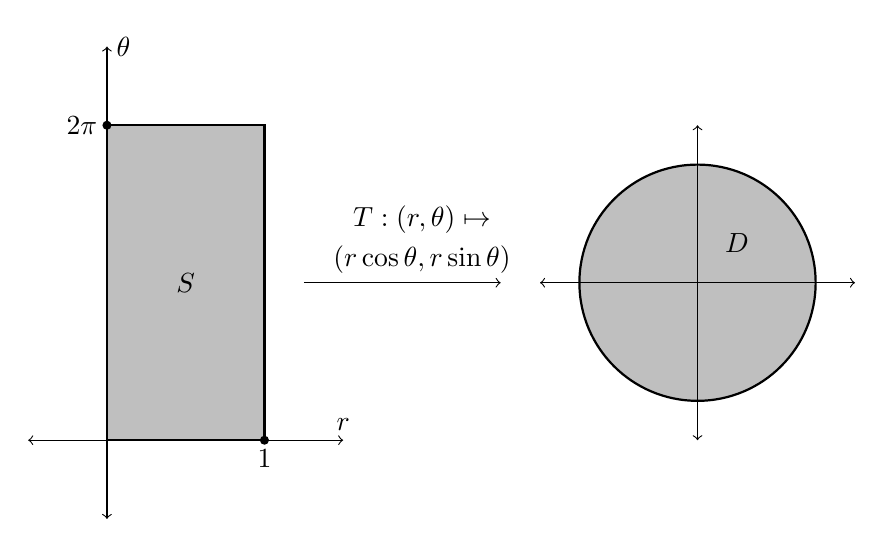
\begin{tikzpicture}
      \draw[thick, fill=lightgray] (7.5,2) circle (1.5);
      \draw[<->] (-1,0)--(3,0);
      \draw[<->] (0,-1)--(0,5);
      \draw[thick, fill=lightgray] (0,0) rectangle (2,4);
      \node at (1,2) {$S$};
      \draw[fill] (0,4) circle (0.05);
      \draw[fill] (2,0) circle (0.05);
      \node[below] at (2,0) {$1$};
      \node[left] at (0,4) {$2 \pi$};
      \node[above] at (3,0) {$r$};
      \node[right] at (0,5) {$\theta$};
      \draw[->] (2.5, 2)--(5,2);
      \node[above] at (4,2.5) {$T: (r, \theta) \mapsto$};
      \node[above] at (4,2) {$ (r \cos{\theta}, r \sin{\theta})$};
      \draw[<->] (5.5,2)--(9.5,2);
      \draw[<->] (7.5,0)--(7.5,4);
      \node at (8,2.5) {$D$};
  \end{tikzpicture}  
  \end{center}
  \end{example}

  \begin{theorem}[Integration over Change of Bases in $\mathbb{R}^n$]
  Let $\mathbb{R}^n$ have the standard orthonormal basis $e_1, e_2, ..., e_n$, and let us construct a new basis $f_1, f_2, ..., f_n$ such that the coefficients of the vectors in $\mathbb{R}^n$ are related with the functions
  \[B: \mathbb{R}^n \longrightarrow \mathbb{R}^n, \;\;\;\; B(u_1, u_2, \ldots, u_n) = \begin{pmatrix}
  x_1 (u_1, \ldots, u_n) \\x_2 (u_1, \ldots, u_n) \\ \vdots \\ x_n (u_1, \ldots, u_n)
  \end{pmatrix}\]
  Given that the region $D \subset \mathbb{R}^n$ is transformed into a new region $S = B(D) \subset \mathbb{R}^n$ under this basis transformation, the integral of function $f(x_1, \ldots, x_n)$ over region $D$ can be expressed as 
  \[\int_D f(x) \, dH = \int_S f \big( x_1(u), x_2(u), ..., x_n (u) \big) \big| J B(u_1, \ldots, u_n)\big| \, d \bar{H}\]
  where the integral on both the left and right hand side represents integration over an $n$-dimensional region, $x$ represents the $n$-tuple $(x_1, \ldots, x_n)$, $u$ represents the $n$-tuple $(u_1, \ldots, u_n)$, and $\big| J B(u_1, \ldots, u_n)\big|$ represents the Jacobian determinant of function $B$. 
  \end{theorem}

  We now describe some common change of basis formulas for polar, cylindrical, and spherical coordinates. 

  \begin{theorem}[Integration in Polar Coordinates]
  \[\iint_{D} f(x, y) \, dx \,dy = \iint_S f(r \cos{\theta}, r \sin{\theta}) r \, dr \, d\theta\]
  \end{theorem}

  \begin{definition}[Cylindrical, Spherical Coordinates]
  In $\mathbb{R}^3$, \textit{cylindrical coordinates} have the following relation to rectangular coordinates. 
  \begin{align*}
      & x = r \cos{\theta} \\
      & y = r \sin{\theta} \\
      & z = z
  \end{align*}
  In $\mathbb{R}^3$, \textit{spherical coordinates} have the following relation to rectangular coordinates. 
  \begin{align*}
      & x = \rho \sin{\phi} \cos{\theta} \\
      & y = \rho \sin{\phi} \sin{\theta} \\
      & z = \rho \cos{\phi}
  \end{align*}
  \end{definition}

  \begin{corollary}[Integration in Cylindrical Coordinates]
  \[\iiint_D f(x, y, z) \, dx \, dy \, dz = \iiint_S f( r \cos{\theta}, r \sin{\theta}, z) r \, dr \, d\theta \, dz\]
  \end{corollary}

  \begin{corollary}[Integration in Spherical Coordinates]
  \[\iiint_D f(x, y, z) \,dx\,dy\,dz = \iiint_S f(\rho \sin{\phi} \cos{\theta}, \rho \sin{\phi} \sin{\theta}, \rho \cos{\phi}) \rho^2 \sin{\theta} \, d\rho \, d\theta \, d\phi\]
  \end{corollary}

  \begin{example}[Gaussian Integral]
  The following is the (un-normalized) probability distribution function of the Gaussian distribution. 
  \[\int_{-\infty}^{\infty} e^{-x^2} \, dx = \sqrt{\pi}\]
  \end{example}

\subsection{Improper Integrals}

  There are generally two types of improper integrals. 
  \begin{enumerate}
    \item The region $D$ integrated over is unbounded. 
    \item The function $f$ that is integrated is unbounded within the region $D$.
  \end{enumerate}

  These types of improper integrals are usually evaluated using a limiting process. When the interval $I$ is unbounded, say $(1, \infty)$, the integral can be evaluated as 
  \[\int_1^\infty \frac{1}{x^2} \,dx = \lim_{b \rightarrow \infty} \int_1^b \frac{1}{x^2} \, dx = \lim_{b\rightarrow \infty} \bigg( 1 - \frac{1}{b} \bigg) = 1\]
  In case 2, we can add a limit at the point where the function $f$ diverges as such. 
  \[\int_0^1 \frac{1}{\sqrt{x}} \, dx = \lim_{a \rightarrow 0} \int_a^1 \frac{1}{\sqrt{x}} \, dx = \lim_{a \rightarrow 0} (2 - 2\sqrt{a}) = 2\]
  We now describe how to integrate over a certain path $p$ embedded in a higher dimensional space $\mathbb{R}^n$, possibly with a scalar or vector field $f$. We must first go over oriented paths. 

  Extending the previous case, we use a multivariate limiting process in $\mathbb{R}^2$. We will first work with case 2, when $f$ is unbounded within the region $D$. Let us define an elementary region $D$ in $\mathbb{R}^2$; without loss of generality, we will make it $y$-simple, meaning that $D$ can be expressed as
    \[D \equiv \{ (x, y) \in \mathbb{R}^2 \; | \; a \leq x \leq b, \; \phi_1 (x) \leq y \leq \phi_2 (x)\}\]
  We can actually assume that the region in which $f$ is unbounded lies in the boundary $\partial D$. This is because if it lied in the interior of $D$, we could split $D$ into pieces across a path that intersects this region with divergent values, evaluate the integrals over the pieces separately, and then sum the integrals. For example, in the rectangular region below, let the dashed line represent the values where the function $f$ diverges. Then, we can split the region into two rectangular regions shown in the right. 
  \begin{center}
  \begin{tikzpicture}
    \draw (0,0) rectangle (3,2);
    \draw[dashed] rectangle (2,0)--(2,2);
    \draw[->] (3.5,1)--(5,1);
    \draw (8,0)--(6,0)--(6,2)--(8,2);
    \draw[dashed] (8,0)--(8,2);
    \draw[dashed] (9,0)--(9,2);
    \draw (9,0)--(10,0)--(10,2)--(9,2);
  \end{tikzpicture}
  \end{center}
  Therefore, assuming that $f$ is unbounded in $\partial D$, we can construct a new region 
  \[D_{\eta, \delta} \equiv \{(x, y) \in \mathbb{R}^2 \; | \; a + \eta \leq x \leq b - \eta, \; \phi_1 (x) + \delta \leq y \leq \phi_2 (x) - \delta\}\]
  for some arbitrarily small numbers $\eta, \delta >0$, meaning that the integral (reduced to iterated integrals using Fubini's theorem) 
  \[F(\eta, \delta) \equiv \iint_{D_{\eta, \delta}} f(x, y) \, dA = \int_{a + \eta}^{b - \eta} \int_{\phi_1 (x) + \delta}^{\phi_2 (x) - \delta} f(x, y) \, dy\,dx\]
  is well defined. 
  \begin{center}
  \begin{tikzpicture}
      \draw[<->] (-0.5,0)--(5,0);
      \draw[<->] (0,-0.5)--(0,5);
      \draw (1,1.5)--(1,3);
      \draw plot [smooth] coordinates {(1,3) (1.5,3.3) (2,3.1) (3,3.8) (4,4.2) (4.5,4)};
      \draw (4.5, 4)--(4.5,1);
      \draw plot [smooth] coordinates {(1,1.5) (2,1.7) (3, 1.6) (3.7, 1.3) ( 4.5,1)};
      \draw[dashed] (1.3,1.85)--(1.3,2.9);
      \draw[dashed] (4.2, 3.8)--(4.2,1.4);
      \draw[dashed] plot [smooth] coordinates {(1.3,2.9) (1.5,3) (2,2.8) (3,3.5) (4,3.9) (4.2,3.8)};
      \draw[dashed] plot [smooth] coordinates {(1.3,1.85) (2,2) (3, 1.9) (3.7, 1.6) ( 4.2,1.4)};
      \node at (3,2.5) {$D_{\eta, \delta}$};
      \node[below left] at (2,1) {$D$};
      \draw[->] (2,1)--(2.5,1.85);
  \end{tikzpicture}
  \end{center}
  Clearly, the function $F( \eta, \delta)$ is a function of two variables $\eta$ and $\delta$. So, if the limit 
  \[\lim_{(\eta, \delta) \rightarrow (0, 0)} F(\eta, \delta)\]
  is well defined, then so is the improper integral. For it to exist, the iterated limits must both equal to a well-defined real number $\mathcal{L}$ (and to each other). That is, 
  \[\lim_{\eta \rightarrow 0} \lim_{\delta \rightarrow 0} F(\eta, \delta) = \lim_{\delta \rightarrow 0} \lim_{\eta \rightarrow 0} F(\eta, \delta) = \mathcal{L} \implies \lim_{(\eta, \delta) \rightarrow (0,0)} F(\eta, \delta) = \mathcal{L}\]


  It is also worthwhile to note that functions unbounded at isolated points can be evaluated using the methods above using a change of basis. Consider the example below. 

  \begin{example}
  In the unit disk $D \subset \mathbb{R}^2$, let the function $f$ be defined as 
  \[f(x, y) \equiv \frac{1}{\sqrt{x^2 + y^2} }\]
  Clearly, $f$ is continuous at every point except $0= (0,0)$, meaning that 
  \[\iint_{D \setminus \{0\}} f(x, y)\, dA\]
  is well-defined. In order to solve the integral over the entire disk, we convert to polar coordinates and evaluate the limit
  \[\iint_{D \setminus \{0\}} f(x, y) \, dA = \lim_{\delta \rightarrow 0} \int_{\delta}^1 \int_0^{2 \pi} r \, f( r \cos{\theta}, r \sin{\theta}) \, d\theta \,dr\]
  \end{example}
  \begin{center}
  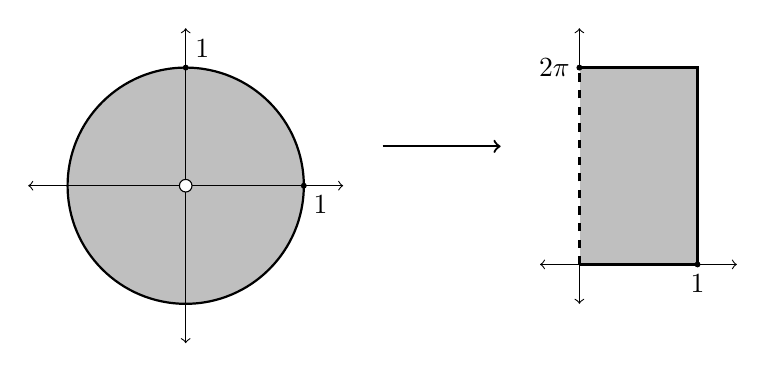
\begin{tikzpicture}
      \draw[thick, fill=lightgray] (0,0) circle (1.5); 
      \draw[<->] (-2,0)--(2,0);
      \draw[<->] (0,-2)--(0,2);
      \draw[fill=white] (0,0) circle (0.08);
      \draw[->, thick] (2.5,0.5)--(4, 0.5); 
      \draw[<->] (4.5,-1)--(7,-1);
      \draw[<->] (5,-1.5)--(5,2);
      \draw[white, fill=lightgray] (5,-1) rectangle (6.5,1.5);
      \draw[thick] (5,-1)--(6.5,-1)--(6.5,1.5)--(5,1.5);
      \draw[thick, dashed] (5,-1)--(5,1.5);
      \draw[fill] (6.5,-1) circle (0.03);
      \node[below] at (6.5,-1) {$1$};
      \node[left] at (5,1.5) {$2 \pi$};
      \draw[fill] (5, 1.5) circle (0.03);
      \draw[fill] (1.5,0) circle (0.03);
      \draw[fill] (0,1.5) circle (0.03);
      \node[below right] at (1.5,0) {$1$};
      \node[above right] at (0,1.5) {$1$};
  \end{tikzpicture}
  \end{center}

  If we are given an unbounded region $D \subset \mathbb{R}^2$, we can first create a bounded region and expand that region using a limit to cover all of $D$. 


